\documentclass{standalone}
\usepackage[dvipsnames,svgnames,x11names]{xcolor}
\usepackage{tikz}
\usepackage{pgfplots}
\pgfplotsset{compat = 1.12}
\usepackage{../thesismath}
\begin{document}
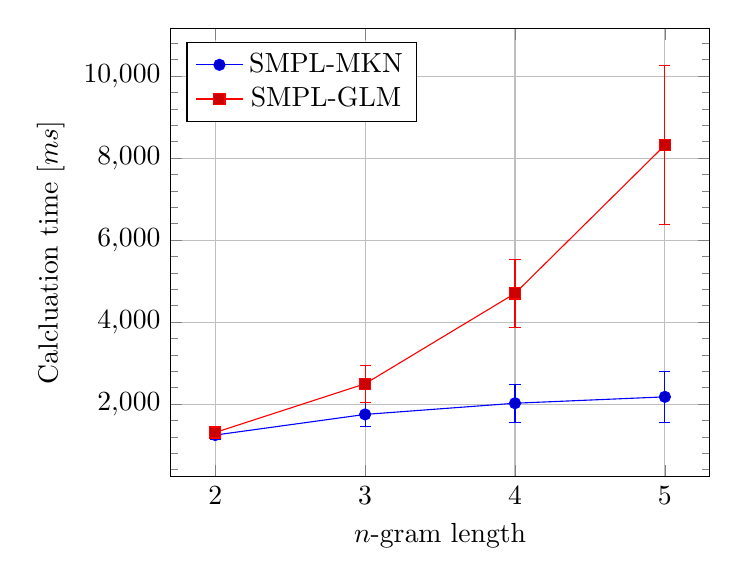
\begin{tikzpicture}[baseline]

\begin{axis}[
  xlabel = {$n$-gram length},
  xtick = {2, ..., 5},
  ylabel = {Calcluation time [$m s$]},
  scaled ticks = false,
  minor y tick num = 4,
  grid = major,
  legend entries = {{SMPL-MKN}, {SMPL-GLM}},
  legend pos = north west,
]

% over 100 test sequences on my own machine

% SMPL-MKN
\addplot+[
  error bars/.cd,
  y dir = both,
  y explicit,
] table [y error = us_error] {
  n us       us_error
  2 1246.684  100.401
  3 1749.752  285.003
  4 2022.604  461.763
  5 2178.157  625.296
};

% SMPL-GLM
\addplot+[
  error bars/.cd,
  y dir = both,
  y explicit,
] table [y error = us_error] {
  n us       us_error
  2 1309.236  100.475
  3 2497.200  452.559
  4 4700.244  823.580
  5 8315.938 1941.474
};

\end{axis}

\end{tikzpicture}
\end{document}
